\setcounter{section}{0}
\section{Hình thành kiến thức mới}

\subsection{Mở đầu}
Hàng ngày, ta thấy bầu trời như là đang quay xung quanh một trục xuyên qua nơi quan sát. Các quan sát chi tiết hơn cho biết, ngoài chuyển động hàng ngày từ phía đông sang phía tây, Mặt Trời còn dịch chuyển so với các sao theo chiều từ phía tây sang phía đông, trọn một vòng hết khoảng một năm. Tại sao ta nhìn thấy bầu trời cũng như Mặt Trời chuyển động như vậy?
\subsection{Hình thành kiến thức mới}
\subsubsection{Đặc điểm cơ bản của chuyển động nhìn thấy}
Dựa trên các quan sát, người ta đã rút ra các đặc điểm cơ bản của chuyển động nhìn thấy của Mặt Trời, Mặt Trăng, Kim Tinh và Thủy Tinh trên nền trời sao như sau:

\begin{minipage}[l]{0.6\textwidth}
	\begin{itemize}
		\item Bầu trời quay xung quanh Trái Đất theo chiều từ phía đông sang phía tây, hết một vòng trong một ngày đêm;
		\item Bên cạnh chuyển động hàng ngày, từ phía đông sang phía tây, Mặt Trời, Mặt Trăng còn dịch chuyển so với các sao theo chiều từ phía tây sang phía đông. So với các sao, Mặt Trời dịch chuyển trọn một vòng trong khoảng 365 ngày; Mặt Trăng dịch chuyển trọn một vòng khoảng 27 ngày;
		\item Hai hành tinh là Thủy Tinh và Kim Tinh luôn ở không quá xa Mặt Trời so với các hành tinh khác trong hệ Mặt Trời. Nhìn từ Trái Đất, chúng ở cách Mặt Trời với các góc tương ứng không quá $28^\circ$ và $48^\circ$.
	\end{itemize}
\end{minipage}
\begin{minipage}[r]{0.4\textwidth}
	\begin{center}
		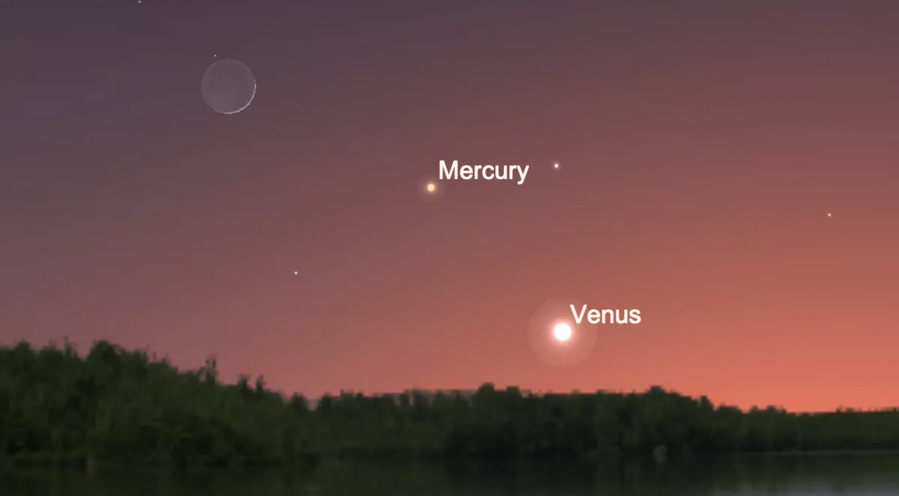
\includegraphics[scale=0.4]{../figs/G10-034-1.png}
	\end{center}
\end{minipage}

\subsubsection{Hệ Mặt Trời}

Mặt Trời là một ngôi sao trong vũ trụ, hình thành cách đây khoảng 4,6 tỉ năm.

Hệ Mặt Trời gồm Mặt Trời, tám hành tinh, các hành tinh lùn, các tiểu hành tinh quay xung quanh Mặt Trời. Các hành tinh không những quay quanh Mặt Trời mà còn tự quay quanh trục của nó.

Tám hành tinh chuyển động quanh Mặt Trời có quỹ đạo gần tròn và mặt phẳng quỹ đạo của chúng khá giống nhau. Trái Đất là hành tinh thứ ba tính từ Mặt Trời. Thời gian Trái Đất quay một vòng xung quanh Mặt Trời là 1 năm.

Thủy Tinh, Kim Tinh, Trái Đất, Hỏa Tinh được gọi là các hành tinh đá. Thiên Vương Tinh, Hải Vương Tinh, Mộc Tinh, Thổ Tinh được gọi là các hành tinh khí.

Hệ Mặt Trời có vành đai tiểu hành tinh nằm giữa quỹ đạo của Hỏa Tinh và Mộc Tinh, được cấu tạo chủ yếu từ đá và kim loại.

\begin{center}
	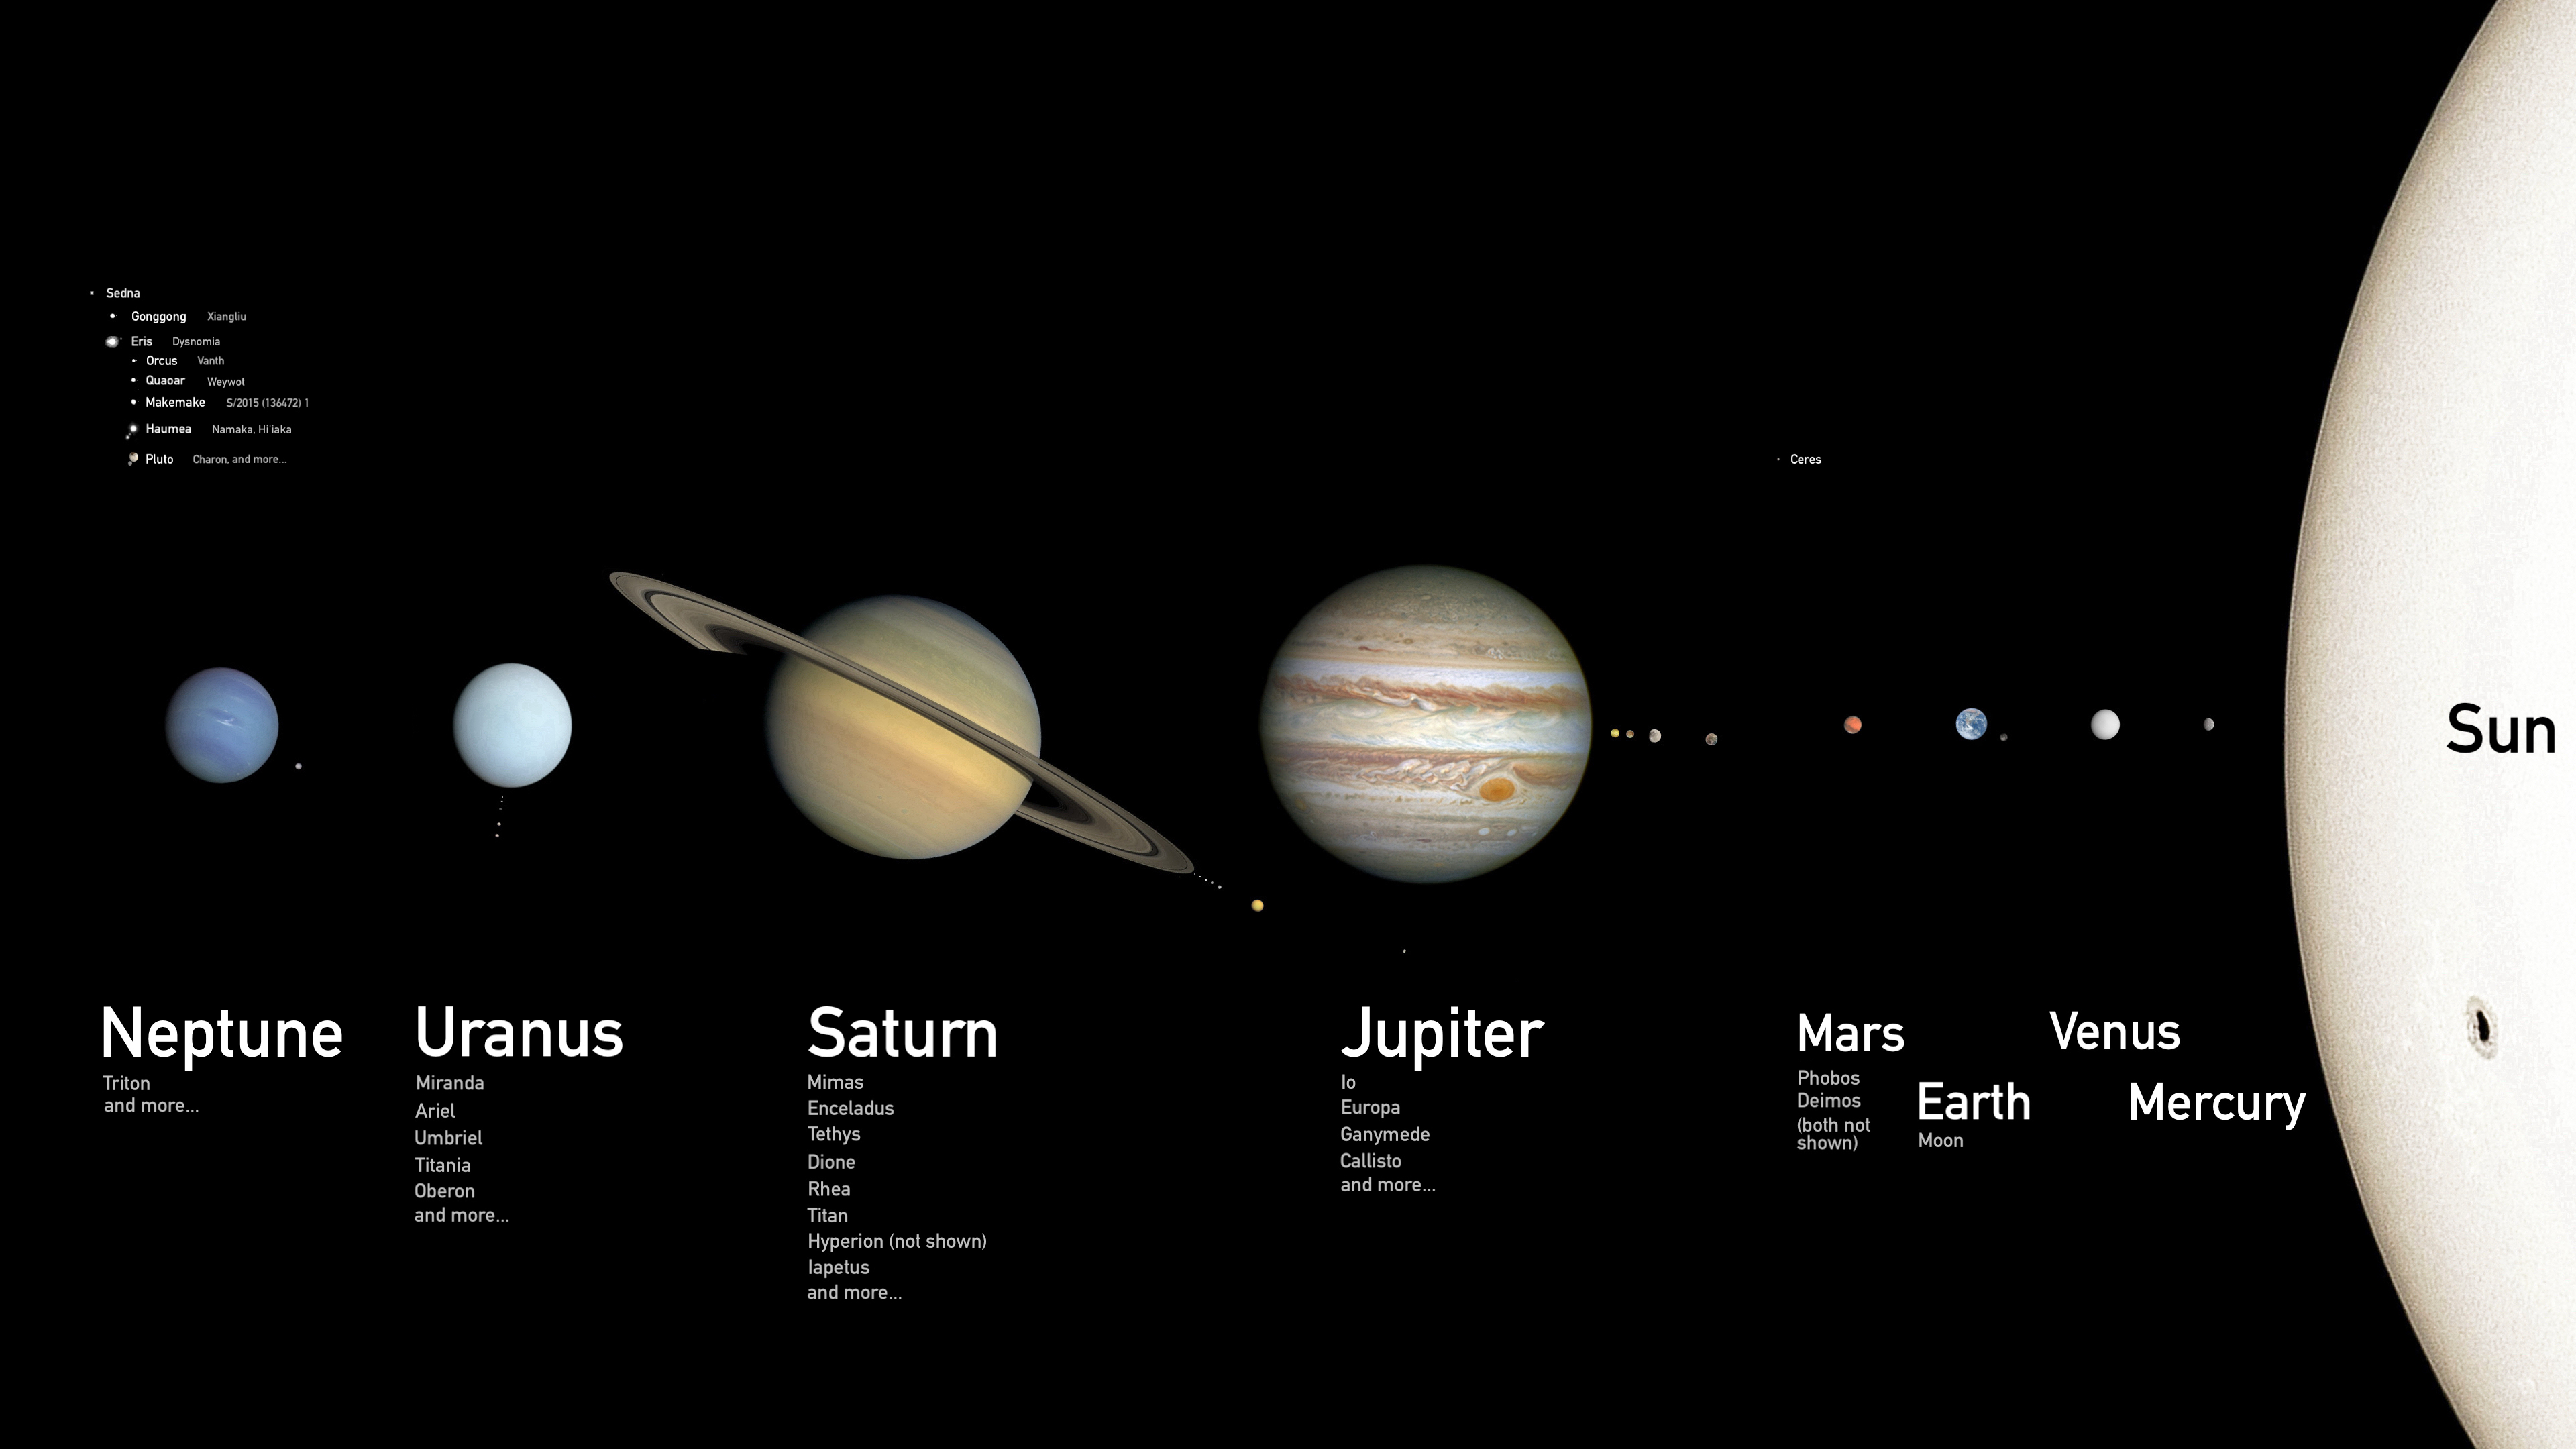
\includegraphics[scale=0.1]{../figs/G10-034-2.jpg}
\end{center}

\subsection{Giải thích một số đặc điểm chuyển động nhìn thấy}
\subsubsection{Giải thích chuyển động nhìn thấy của bầu trời}
Chúng ta đã biết Trái Đất quay quanh trục theo chiều từ phía tây sang phía đông. Vì quan sát bầu trời từ Trái Đất đang quay nên ta thấy bầu trời quay theo chiều ngược lại, hết một vòng trong một ngày đêm, đúng bằng thời gian Trái Đất quay quanh trục hết một vòng.

\begin{center}
	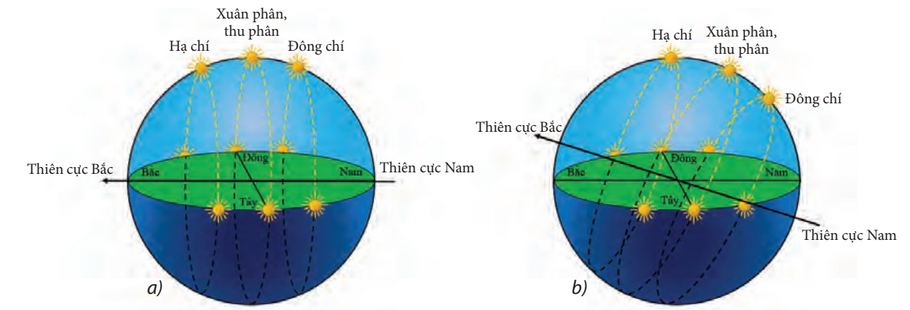
\includegraphics[scale=0.9]{../figs/G10-034-3.png}
\end{center}

\subsubsection{Giải thích chuyển động nhìn thấy của Mặt Trời}
\begin{minipage}[l]{0.6\textwidth}
	Do Trái Đất tự quay quanh trục theo chiều từ tây sang đông, đồng thời quay quanh Mặt Trời nên ta có cảm giác Mặt Trời chuyển động xung quanh Trái Đất. Tại một nơi trên Trái Đất, ta thấy Mặt Trời mọc lên ở hướng đông và lặn ở hướng tây. Quỹ đạo chuyển động biểu kiến của Mặt Trời trong một năm gọi là Hoàng Đạo.
	
	Thực tế, trong một năm, Mặt Trời chỉ mọc đúng chính Đông và lặn đúng chính Tây vào 2 ngày: xuân phân (21/03) và thu phân (23/09). Sau xuân phân, điểm mọc của Mặt Trời lệch dần về phía Đông Bắc (điểm lặn lệch dần về phía Tây Bắc), ngày lệch cực đại là hạ chí (22/06). Qua thu phân, điểm mọc của Mặt Trời lệch dần về phía Đông Nam (điểm lặn lệch dần về phía Tây Nam), ngày lệch cực đại là dông chí (22/12).
\end{minipage}
\begin{minipage}[r]{0.4\textwidth}
	\begin{center}
		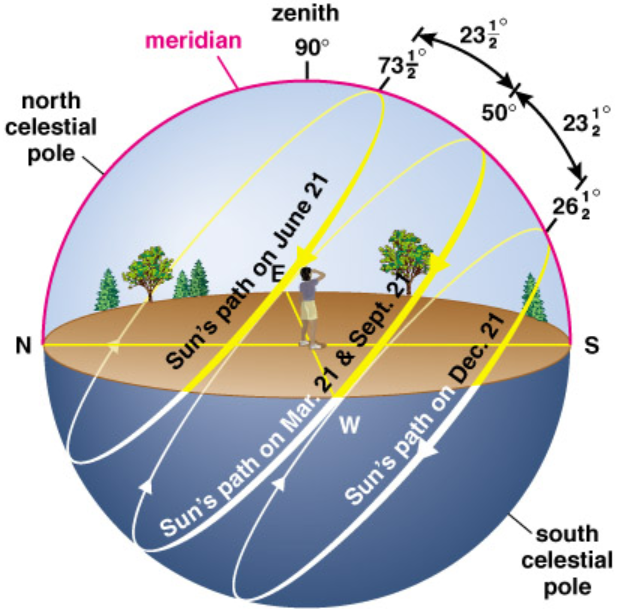
\includegraphics[scale=0.5]{../figs/G10-034-4.png}
	\end{center}
\end{minipage}

\subsection{Mở rộng}
\subsubsection{Giải thích chuyển động nhìn thấy của Mặt Trăng}
Một chu kì của Mặt Trăng bắt đầu từ ngày ta không thấy trăng. Những ngày sau, Mặt Trăng có hình dạng lưỡi liềm, to dần và có hình bán nguyệt phải vào khoảng ngày 7 hoặc 8 của Tuần Trăng (độ dài trung bình của một tháng Âm lịch, khoảng 29,5 ngày). Mặt Trăng tiếp tục tròn dần đến khi trăng tròn đầy vào khoảng hai tuần kể từ đầu Tuần Trăng (ngày 14 hoặc 15). Tiếp sau đó, Mặt Trăng bị khuyết dần, trở về hình bán nguyệt trái, sau đó thành hình lưỡi liềm trái và cuối cùng trở về kì không trăng.

Ánh sáng của Mặt Trăng có được là do Mặt Trăng phản xạ ánh sáng từ Mặt Trời. Trên thực tế, lúc nào Mặt Trăng cũng hiện diện, nhưng ta chỉ có thể quan sát thấy phần Mặt Trăng được Mặt Trời chiếu sáng và hướng về phía Trái Đất. Ngoài ra, chu kì tự quay quanh trục của Mặt Trăng đúng bằng chu kì quay của Mặt Trăng quanh Trái Đất, nên ta chỉ có thể quan sát một nửa bề mặt của Mặt Trăng hướng về Trái Đất.

\begin{center}
	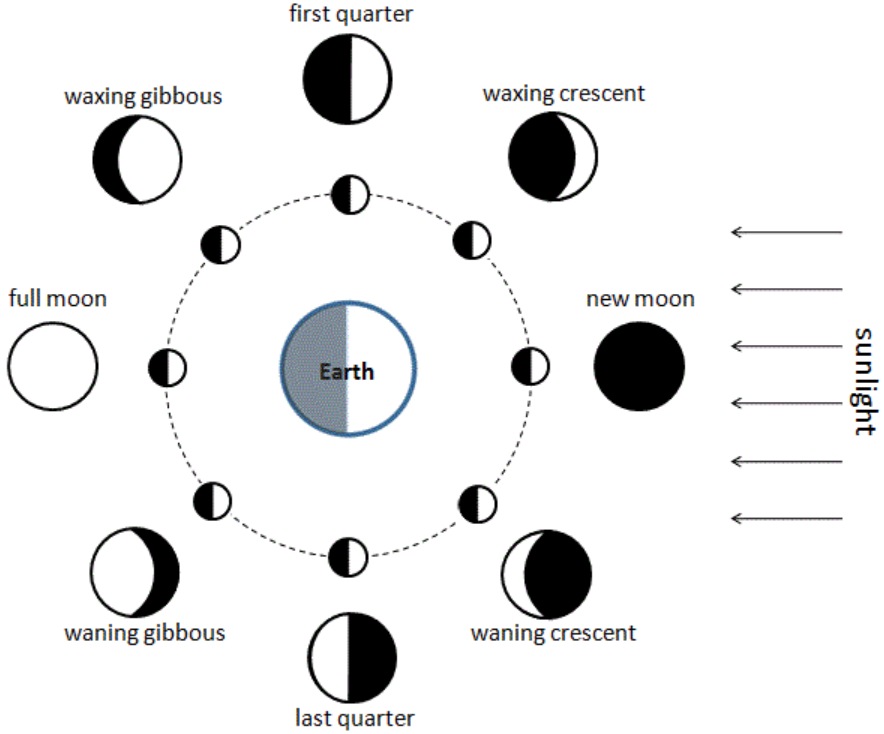
\includegraphics[scale=0.5]{../figs/G10-034-5}
\end{center}
\subsubsection{Giải thích chuyển động nhìn thấy của Kim Tinh và Thủy Tinh}
Thủy Tinh và Kim Tinh mọc và lặn gần như cùng lúc với Mặt Trời. Thủy Tinh thường mọc trước hoặc lặn sau Mặt Trời khoảng 2 giờ, Kim Tinh là 4 giờ. Khi Mặt Trời đang ở đường chân trời, góc lệch (li giác) cực đại khi ta quan sát Thủy Tinh và Kim Tinh so với Mặt Trời có giá trị lần lượt khoảng $28^\circ$ và $48^\circ$.

Khi quan sát trên nền trời sao, Kim Tinh là thiên thể sáng nhất trên bầu trời đêm sau Mặt Trăng. Kim Tinh còn được gọi là Sao Mai (do mọc trước Mặt Trời) và Sao Hôm (do lặn sau Mặt Trời).

Thông thường, Kim Tinh và Thủy Tinh di chuyển từ Đông sang Tây, nhưng đôi khi chúng đổi chiều chuyển động từ Tây sang Đông. Sự đổi chiều chuyển động của Kim Tinh và góc dời cực đại khi quan sát từ Trái Đất có thể được giải thích bởi mô hình hệ nhật tâm của Copernicus.

\section{Mục tiêu bài học - Ví dụ minh họa}
\begin{dang}{Nêu được các đặc điểm cơ bản của Hệ Mặt Trời}
	\viduii{2}{Hãy nêu một số đặc điểm cơ bản của Hệ Mặt Trời.
	}
	{	\begin{center}
			\textbf{Hướng dẫn trả lời}
		\end{center}
		
		Mặt Trời là một ngôi sao trong vũ trụ, hình thành cách đây khoảng 4,6 tỉ năm.
		
		Hệ Mặt Trời gồm Mặt Trời, tám hành tinh, các hành tinh lùn, các tiểu hành tinh quay xung quanh Mặt Trời. Các hành tinh không những quay quanh Mặt Trời mà còn tự quay quanh trục của nó.
		
		Tám hành tinh chuyển động quanh Mặt Trời có quỹ đạo gần tròn và mặt phẳng quỹ đạo của chúng khá giống nhau. Trái Đất là hành tinh thứ ba tính từ Mặt Trời. Thời gian Trái Đất quay một vòng xung quanh Mặt Trời là 1 năm.
		
		Thủy Tinh, Kim Tinh, Trái Đất, Hỏa Tinh được gọi là các hành tinh đá. Thiên Vương Tinh, Hải Vương Tinh, Mộc Tinh, Thổ Tinh được gọi là các hành tinh khí.
		
		Hệ Mặt Trời có vành đai tiểu hành tinh nằm giữa quỹ đạo của Hỏa Tinh và Mộc Tinh, được cấu tạo chủ yếu từ đá và kim loại.
	}
	\viduii{2}{Dựa vào đặc điểm các hành tinh trong Hệ Mặt Trời, hãy trả lời các câu hỏi sau:
		\begin{enumerate}[label=\alph*)]
			\item Hành tinh nào gần Mặt Trời nhất?
			\item Hành tinh nào có nhiệt độ trung bình năm cao nhất?
			\item Hành tinh nào có kích thước lớn nhất?
			\item Hành tinh nào có khối lượng lớn nhất?
			\item Hành tinh nào có đặc điểm địa hình gần giống Trái Đất nhất?
			\item Hành tinh nào quay ngược chiều so với các hành tinh còn lại?
		\end{enumerate}
	}
	{	\begin{center}
			\textbf{Hướng dẫn trả lời}
		\end{center}
		
		\begin{enumerate}[label=\alph*)]
			\item Hành tinh nào gần Mặt Trời nhất?
			
			Thủy Tinh (Mercury)
			\item Hành tinh nào có nhiệt độ trung bình năm cao nhất?
			
			Kim Tinh (Venus)
			
			\item Hành tinh nào có kích thước lớn nhất?
			
			Mộc Tinh (Jupiter)
			\item Hành tinh nào có khối lượng lớn nhất?
			
			Mộc Tinh (Jupiter)
			
			\item Hành tinh nào có đặc điểm địa hình gần giống Trái Đất nhất?
			
			Hỏa Tinh (Mars)
			
			\item Hành tinh nào quay ngược chiều so với các hành tinh còn lại?
			
			Kim Tinh (Venus)	
		\end{enumerate}
		
	}
\end{dang}
\begin{dang}{Giải thích một số đặc điểm chuyển động nhìn thấy\\ của Mặt Trời, Mặt Trăng, Kim Tinh và Thủy Tinh}
	\viduii{2}{Hãy giải thích chuyển động nhìn thấy của Mặt Trời.
	}
	{	\begin{center}
			\textbf{Hướng dẫn trả lời}
		\end{center}
		
		Do Trái Đất tự quay quanh trục theo chiều từ Tây sang Đông, đồng thời quay quanh Mặt Trời. Do đó, tại một nơi trên Trái Đất, ta thấy Mặt Trời mọc lên ở hướng Đông và lặn ở hướng Tây.
		
	}
	\viduii{2}{Hãy giải thích chuyển động nhìn thấy của Mặt Trăng.
	}
	{	\begin{center}
			\textbf{Hướng dẫn trả lời}
		\end{center}
		
		Trái Đất quay quanh Mặt Trời, trong khi Mặt Trăng chuyển động quanh Trái Đất trên quỹ đạo gần tròn với chu kỳ quay là 1 Tuần trăng. Tùy vị trí tương đối của Mặt Trời, Mặt Trăng và Trái Đất, ta sẽ thấy được những hình dạng khác nhau của Mặt Trăng, tương ứng với các pha khác nhau:
		\begin{itemize}
			\item Trăng mới: Mặt Trăng có thời gian mọc và lặn trùng với Mặt Trời nên chúng ta không thể quan sát được Mặt Trăng ở Trái Đất. Những ngày tiếp theo, Mặt Trăng dịch chuyển trên quỹ đạo của nó quanh Trái Đất và có dạng lưỡi liềm (trăng non) khi được quan sát từ Trái Đất.
			\item Thượng Huyền (bán nguyệt đầu tháng): Tại Bắc bán cầu, ta sẽ thấy được Mặt Trăng có dạng hình bán nguyệt có đỉnh nằm ở hướng Nam vào hoàng hôn và lặn dần về phía Tây vào lúc nửa đêm.
			\item Trăng tròn: Mặt Trăng phản xạ toàn bộ ánh sáng Mặt Trời nên ở phần tối của Trái Đất sẽ thấy trăng tròn cả đêm.
			\item Hạ Huyền (bán nguyệt cuối tháng): Mặt Trăng có hình bán nguyệt nhưng ngược bên với pha Thượng Huyền. Ngoài ra, ta quan sát được Mặt Trăng lên đến đỉnh bầu trời vào lúc nửa đêm và lặn khi bình minh. Những ngày tiếp theo, trăng khuyết dần và và trở về thời kì không trăng để tiếp tục một chu kì mới.
		\end{itemize}
		
	}
	\viduii{2}{Hãy giải thích chuyển động nhìn thấy của Kim Tinh, Thủy Tinh.
	}
	{	\begin{center}
			\textbf{Hướng dẫn trả lời}
		\end{center}
		
		Kim Tinh và Trái Đất cùng quay quanh Mặt Trời trên quỹ đạo gần như tròn và gần như đồng phẳng với nhau. Do quỹ đạo của Kim Tinh quanh Mặt Trời có bán kính nhỏ hơn quỹ đạo của Trái Đất quanh Mặt Trời nên Kim Tinh chuyển động với tốc độ góc lớn hơn tốc độ góc của Trái Đất. Trường hợp Kim Tinh lặn sau Mặt Trời, Kim Tinh được gọi là Sao Hôm. Trường hợp Kim Tinh xuất hiện trước Mặt Trời vào lúc bình minh, Kim Tinh được gọi là Sao Mai.
		
		Chuyển động của Thủy Tinh trong Hệ Mặt Trời hoàn toàn tương tự như chuyển động của Kim Tinh. Tuy nhiên, do kích thước của Thủy Tinh nhỏ hơn Kim Tinh và xa Trái Đất hơn nên ta khó quan sát được Thủy Tinh trên bầu trời bằng mắt thường.
		
	}
\end{dang}
\section{Tự luận}
\begin{enumerate}[label=\bfseries Câu \arabic*:]
	\item \mkstar{1}
	
	
	{
		Hãy kể tên các hành tinh trong hệ Mặt Trời.
	}
	
	\hideall
	{
		1. Thủy tinh.
		
		2. Kim tinh.
		
		3. Trái Đất.
		
		4. Hỏa tinh.
		
		5. Mộc tinh.
		
		6. Thổ tinh.
		
		7. Thiên Vương tinh.
		
		8. Hải Vương tinh.
	}
	\item \mkstar{2}
	
	{
		Hãy nêu cấu trúc của hệ Mặt Trời và sự chuyển động của các hành tinh trong hệ Mặt Trời.
	}
	
	\hideall{
		
		Hệ Mặt Trời gồm Mặt Trời, tám hành tinh, các hành tinh lùn, các tiểu hành tinh quay xung quanh Mặt Trời. Các hành tinh không những quay xung quanh Mặt Trời mà còn tự quay quanh mình nó.
		
		Tám hành tinh chuyển động quanh Mặt Trời có quỹ đạo gần tròn và mặt phẳng quỹ đạo của chúng gần như trùng khít với nhau.
	}
	
	\item \mkstar{2}
	
	
	{
		Hãy nêu đặc điểm cấu tạo của một số hành tinh trong hệ Mặt Trời.
	}
	
	\hideall
	{
		Thủy tinh, Kim tinh, Trái Đất, Hỏa tinh được gọi là các hành tinh đá do chúng có thành phần cấu tạo chủ yếu từ đá và kim loại.
		
		Thiên Vương tinh, Hải Vương tinh, Mộc tinh, Thổ tinh được gọi là các hành tinh khí, có khối lượng lớn hơn rất nhiều so với Thủy tinh, Kim tinh, Trái Đất, Hỏa tinh.
		
		Mộc tinh và Thổ tinh là hai hành tinh lớn nhất trong hệ Mặt Trời. Thành phần cấu tạo của nó chủ yếu là từ khí helium và khí hydrogen.
		
		Thiên Vương tinh và Hải Vương tinh có thành phần chính từ băng, nước, ammonia và methane.
	}
	\item \mkstar{2}
	

	{
		Mô tả và kể tên hình dạng Mặt Trăng quan sát thấy từ Trái Đất.
	}
	
	\hideall
	{
		Mặt Trăng là vệ tinh tự nhiên duy nhất của Trái Đất. Từ Trái Đất quan sát thấy Mặt Trăng cũng mọc hướng Đông và lặn hướng Tây như Mặt Trời.
		
		Mặt Trăng vào ngày rằm là tròn nhất.
	}
	\item \mkstar{2}
	

	{
		Dựa vào chiều quay của Trái Đất, hãy thảo luận để rút ra kết luận về chiều chuyển động và sự mọc, lặn của Mặt Trời hằng ngày.
	}
	
	\hideall
	{
		Nếu đứng nhìn về hướng Bắc, hằng ngày chúng ta sẽ thấy Mặt Trời mọc ở phía Đông và lặn ở phía Tây hay mọc bên tay phải và lặn bên tay trái. 
		
		Đường đi của Mặt Trời cao dần từ mùa đông đến mùa hạ. Mùa hạ, Mặt Trời ở vị trí cao nhất trên hướng chính Nam.
	}
	\item \mkstar{3}
	
	
	{
		Dựa vào đường đi của Mặt Trời quan sát thấy trên Trái Đất, hãy thảo luận để giải thích câu sau: "Đêm tháng năm chưa nằm đã sáng. Ngày tháng mười chưa cười đã tối".
	}
	
	\hideall
	{
		Đêm tháng 5 chưa nằm đã sáng, ngày tháng 10 chưa cười đã tối". Từ trong thực tế hiện tượng "Ngày dài, đêm ngắn" (tháng 5) và "Ngày ngắn, đêm dài" (tháng 10) do ảnh hưởng sự tự quay quanh trục của Trái Đất và chuyển động của TĐ quanh Mặt Trời nên sinh ra hiện tượng ngày đêm chênh lệch giữa 2 nửa cầu và các mùa. - Vào tháng 6 (tháng 5 âm lịch): Do trục TĐ nghiêng và hướng nghiêng ko đổi, ánh sáng MT chỉ chiếu đc một nửa TĐ (do TĐ hình cầu), nửa cầu Bắc ngả về phía MT nó được chiếu sáng nhiều hơn nửa cầu Nam nân các địa điểm trên nửa cầu Bắc có ngày dài hơn đêm (ngày dài, đêm ngắn). Nước ta nằm ở nửa cầu Bắc do đó đêm tháng 5 ngắn, đúng với câu nói của nhân dân ta: "Đêm tháng 5 chưa nằm đã sáng" - Vào tháng 12 (tháng 10 âm lịch): Vào mùa đông, do nửa cầu Bắc chếch xa MT nên các địa điểm trên nửa cầu Bắc có ngày ngắn đêm dài. Nước ta nằm ở nửa cầu Bắc do đó ngày ở tháng 10 ngắn đúng với lời nói "Ngày tháng 10 chưa cười đã tối".
	}
	\item \mkstar{2}
	
	{
		Thảo luận để rút ra kết luận về sự chuyển động của Mặt Trăng quanh Trái Đất.
	}
	
	\hideall{
		
		Mặt Trăng xoay quanh Trái Đất với chu kì là 29,5 ngày và chuyển động cùng Trái Đất xung quanh Mặt Trời. Ngoài chuyển động quanh Trái Đất, Mặt Trăng cũng tự quay xung quanh mình nó và chu kì bằng chu kì quay quanh Trái Đất, nên Mặt Trăng luôn hướng một mặt duy nhất về phía Trái Đất.
	}
	
	
	\item \mkstar{3}
	

	{
		Hãy so sánh mô hình hệ địa tâm của Plotemy và hệ nhật tâm của Copernic về sự chuyển động của các hành tinh, vị trí của các hành tinh. Nêu hạn chế của mô hình nhật tâm so với mô hình hệ Mặt Trời ngày nay.
	}
	
	\hideall
	{
		Hệ địa tâm của Plotemy: Các hành tinh quay xung quanh Trái Đất.
		
		Hệ nhật tâm của Copernicus, lấy Mặt Trời làm trung tâm, các hành tinh quay xung quanh Mặt Trời trên quỹ đạo tròn.
		
		Khác với mô hình Copernicus, ngày nay hệ Mặt Trời không phải chỉ có 6 hành tinh mà gồm 8 hành tinh. Mặt khác, các hành tinh quay xung quanh Mặt Trời không phải theo quỹ đạo tròn mà là gần tròn (quỹ đạo elip). Mặt Trăng cũng quay xung quanh Trái Đất theo quỹ đạo elip.
	}
	\item \mkstar{2}
	

	{
		Mô tả chuyển động nhìn thấy của Mặt Trời mà bạn biết.
	}
	
	\hideall
	{
		Mặt Trời quay xung quanh Trái Đất theo chiều từ phía đông sang phía tây, hết một vòng trong một ngày đêm.
		
		Bên cạnh chuyển động hằng ngày, từ phía đông sang phía tây, Mặt Trời, Mặt Trăng còn dịch chuyển so với các sao theo chiều từ phía tây sang phía đông. So với các sao, Mặt Trời dịch chuyển trọn một vòng trong khoảng 365 ngày.
		
	}
	\item \mkstar{2}
	
	
	{
		Nêu sự khác biệt giữa chuyển động của Kim tinh và Thủy tinh so với chuyển động của Mặt Trăng. 
	}
	
	\hideall
	{
		Thủy tinh thường mọc trước hoặc lặn sau Mặt Trời khoảng 2 giờ, trong khi Kim tinh thường mọc trước hoặc lặn sau Mặt Trời khoảng 4 giờ. 
		
		Kim tinh và Thủy tinh không phát sáng mà chỉnh phản chiếu ánh sáng từ Mặt Trời chiếu đến, nên luôn có một nửa được chiếu sáng và một nửa trong bóng tối. 
		
		Khi quan sát trên nền sao, Kim tinh là thiên thể sáng nhất trên bầu trời đêm sau Mặt Trăng. Kim tinh đạt độ sáng lớn nhất ngay sát thời điểm bình minh hoặc hoàng hôn và vì vậy thường được gọi là Sao Mai và Sao Hôm.
	}
\end{enumerate}